\documentclass[border=10pt]{standalone}
\usepackage{pgfplots}
\pgfplotsset{compat=1.18}
\begin{document}
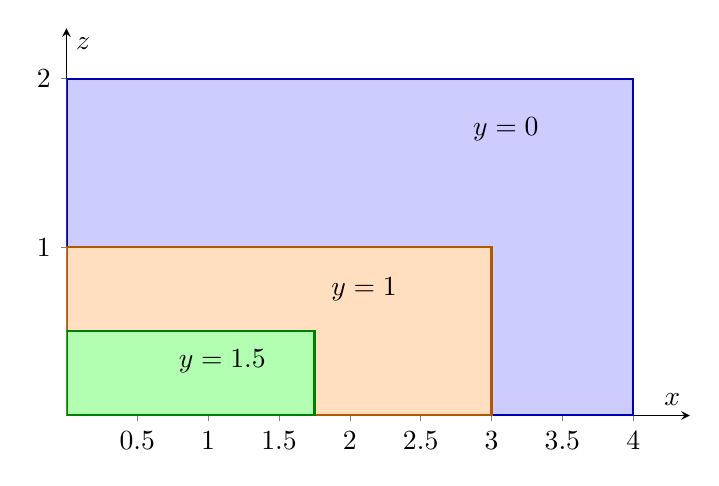
\begin{tikzpicture}
\begin{axis}[
    axis lines=middle,
    xlabel=$x$, ylabel=$z$,
    xmin=0, xmax=4.4, ymin=0, ymax=2.3,
    width=9.5cm, height=6.5cm,
    ]
% y=0
\addplot[fill=blue!20, draw=blue!70!black, thick, domain=0:4] {2} \closedcycle;
% y=1
\addplot[fill=orange!25, draw=orange!70!black, thick, domain=0:3] {1} \closedcycle;
% y=1.5
\addplot[fill=green!30, draw=green!50!black, thick, domain=0:1.75] {0.5} \closedcycle;
\node at (axis cs:1.1,0.32) {$y=1.5$};
\node at (axis cs:2.1,0.75) {$y=1$};
\node at (axis cs:3.1,1.7) {$y=0$};
\end{axis}
\end{tikzpicture}
\end{document}